% 
% Document: NESD 2013 Final Report
% Author: Matthew Gidden
% Date: Sept. 10, 2013
% Notes: Andrew Cartas provided an initial Latex draft 
%        for his UF report, which was used as a template.
% 

\documentclass[12pt]{article}

%%%%%% preamble %%%%%%%%%%
\usepackage{amssymb}
\usepackage{amsmath}
\usepackage{amsthm}
\usepackage[left=1in,top=1in,bottom=1in,right=1in]{geometry}
\usepackage[pdftex]{graphicx}
\usepackage{indentfirst}
\usepackage{subcaption}
\usepackage{setspace}


%%%%%%%%%%%%%%%%%%%%%%%%%%%%%%%%%%%%%%%%%%%%%%%%
\begin{document}

%%%%%% titlepage %%%%%%%%%%
%% title.tex
%% Copyright 2013 M. J. Gidden

% This program can redistributed and/or modified under the terms
% of the LaTeX Project Public License Distributed from CTAN
% archives in directory macros/latex/base/lppl.txt; either
% version 1 of the License, or (at your option) any later version.

\begin{center}
\begin{figure}[hbtp]
\centering
\includegraphics*[scale=1]{NESD_Logo.png}
\end{figure}
\begin{LARGE}
Nuclear Engineering Student Delegation\\
July 6-12, 2013\\
Final Report

\vspace{.5cm}
\end{LARGE}
\end{center}
\begin{large}
\begin{minipage}[b]{0.45\linewidth}
\centering
\begin{tabular}{r}
Matthew Gidden (Chair)\\
Mark Reed (Co-Vice Chair)\\
Nicholas Thompson (Co-Vice Chair)\\ 
Shelly Arreguin\\
Samuel Brinton\\
Lane Carasik\\
Andrew Cartas \\
Erin Dughie\\
Tom Grimes\\
Thomas Holschuh\\
Anagha Iyengar\\
Buckley ODay\\
Ekaterina Paramonova\\
Vishal Patel\\
Jeremy Pearson\\
Benjamin Reinke\\
\end{tabular}
\end{minipage}
\hspace{1cm}
\begin{minipage}[b]{0.45\linewidth}
\centering
\begin{tabular}{l}
University of Wisconsin-Madison\\
Massachusetts Institute of Technology\\
Rensselaer Polytechnic Institute\\
University of Washington, Seattle\\
Massachusetts Institute of Technology\\
Texas A\&M University\\
University of Florida\\
University of New Mexico\\
Purdue University\\
Oregon State University\\
University of Tennessee\\
Massachusetts Institute of Technology\\
Massachusetts Institute of Technology\\
Texas A\&M University\\
University of California, Irvine\\
The Ohio State University\\
\end{tabular}
\end{minipage}
\end{large}
\thispagestyle{empty}


\newpage
\tableofcontents
\thispagestyle{empty}

\newpage
\setcounter{page}{1} 

\section{Introduction}

The Washington Nuclear Engineering Student Delegation (NESD) is an independently
organized program with the goal of allowing students studying nuclear science
and engineering to acquire hands-on experience with the political process to
learn how they can make a positive impact on the future of nuclear energy,
policy, education, and research. The Delegation was formed in 1994 in response
to the elimination of nuclear research reactor program funding in the FY 1995
budget. Funding was reinstated as a direct result of students' interactions with
lawmakers. Owing to the success of the first endeavor, return trips were
organized every year since.

Since the founding of the Delegation, there have been over 75 delegates from 21
of the nation's most prestigious universities. Over the years, these delegates
have met with many senators, congressmen, the Secretary of Energy, the Adviser
to the President on Science and Technology Policy, several NRC commissioners,
staff from the Senate and House Energy Committees, presidents and CEOs of
companies, and other industry leaders and policymakers. The delegation continues
to express the views of the student population on nuclear science and
engineering education. This years delegation was comprised of sixteen students
from 12 universities across the nation.

Each year, the Delegation convenes in Washington and for a day formulates a set
of policy statements that convey their views on nuclear energy, education, and
research. Then, for the following three days, they meet with policymakers on
Capitol Hill to deliberate over the subjects they have identified. Because many
of the policymakers and staff on Capitol Hill do not have a technical
background, it is important that the members of the Delegation inform them of
how students across the nation feel on relevant issues.

\begin{figure}[hbtp]
\centering
\caption{NESD at the White House}
\includegraphics*[scale=.4]{NESD_WH.jpg}
\end{figure}

\newpage

\section{Executive Summary}

The Nuclear Engineering Student Delegation marked another successful trip in
July 2013.  Delegates had unforgettable experiences learning about, and
participating in the policymaking process.

A focus of the 2013 delegation was to meet with Senate offices to encourage
support for the Integrated University Program.  At the time of the Delegation,
the House Energy and Water appropriations bill had passed, with funding for IUP
included.  The Senate bill, which did not include IUP funding, had left
committee but not yet reached the floor for a vote.

Each NESD is a new and unique delegation. For the first time, the 2013
Delegation had meetings the Department of State and four NRC Commissioners,
including Chairman Macfarlane.  In addition, in keeping with at least the past
two delegations, the 2013 NESD met with NEI senior staff, executive branch
officials from DOE (including Assistant Secretary for Nuclear Energy Pete
Lyons), Office of Management and Budget (OMB), NRC, Annie Caputo- a Professional
Staff member at House Energy and Commerce Committee and the United States House
of Representatives, and the current ANS fellow Vincint Esposito.  The main
efforts of the Delegates were spent meeting with Members of Congress and their
staffers; the NESD was successful in meeting with or submitting policy
statements to every Senate office and a sizable number of House offices.

The 2013 NESD was successful in its twin purposes – to educate and inspire a
group of talented, young nuclear engineers about the policy-making world of
Washington, DC; and to convey the thoughts, opinions, and interests of nuclear
engineering students to policymakers.  It was an experience none of the
delegates will soon forget, and we are extremely grateful for the support we
received from NEI, ANS, and everyone who took time to meet with us.

\newpage
\section{2013 Schedule}

\textbf{Saturday, July 6th- Arrival}
\begin{itemize}
\item 7:00pm - 9:00pm - Orientation Dinner
\end{itemize}

\textbf{Sunday, July 7th}
\begin{itemize}
\item 8:30am - 6:00pm - Policy statement drafting
\item 7:30pm - 9:30pm - Dinner
\end{itemize}

\textbf{Monday, July 8th}
\begin{itemize}
\item 9:00am - 1:30pm - AREVA Meeting
\item 2:00pm - 5:00pm - NEI Meeting
\item 6:30pm - 9:00pm - Dinner with Lara Pierpoint
\end{itemize}

\textbf{Tuesday, July 9th}
\begin{itemize}
\item 9:00am -11:30am - DOE Meeting
\item 12:00pm- 1:30pm - Lunch with Pete Lyons
\item 2:00pm - 6:00pm - NRC Commissioner Meeting
\item 7:00pm - 9:00pm - Congressional Strategy Session and Student Mixer
\end{itemize}

\textbf{Wednesday, July 10th}
\begin{itemize}
\item 9:00am -12:00pm - Department of State meeting with Gilbert Brown
\item 12:00pm- 3:00pm - Lunch at National Academy of Sciences and congressional
  strategy session
\item 4:00pm - 5:00pm - OMB Meeting with Christine MacDonald
\item 6:00pm - 8:30pm - Dinner with NRC Commissioner Bill Magwood
\end{itemize}

\textbf{Thursday, July 11th}
\begin{itemize}
\item 8:00am - 5:00pm - Congressional Hill Visits
\item 6:30pm - 8:30pm - Dinner with Annie Caputo and Vincint Esposito (ANS
  Fellow)
\end{itemize}

\textbf{Friday, July 12th - Departure}
\begin{itemize}
\item 8:00am - 5:00pm - Congressional Hill Visits
\end{itemize}

\newpage
\section{Policy Statement Writing}

The entire group gathered in a meeting room at the hotel and spent the first
hour or so talking about what they considered to be the important issues facing
nuclear engineering education. After everyone had a chance to express their
thoughts, the Chairs gave a quick recap of everything that had been
discussed. The group decided on five general categories on which to focus the
policy statement, and delegates chose which area they wanted to help write. The
delegates met in teams and came up with outlines for their respective sections
of the policy statement before lunch. The delegates chose to concentrate on
issues such as the federal governments role in hiring nuclear science
professionals, the role of the federal government in funding the Integrated
University Program, their role in the Nuclear Energy University Partnership, and
their role in basic university nuclear infrastructure investment.

After the break for lunch, the delegates divided back into groups and drafted
the five sections. At the end of the day the group edited the sections
together. The delegates read the combined document agreed upon its content by
consensus. The chairs continued editing for grammar, etc. throughout the
evening, but no major content changes were made without the entire group. The
group then reviewed the final product. 


\newpage
\section{Meetings}

Over the course of the week, the Delegates were privileged to attend meetings
with key people from the nuclear industry and the Executive and Legislative
branches.  Each meeting provided the delegates with new information and
perspectives on various aspects of nuclear energy, education, and policy.  Some
highlights from meetings that were new this year are discussed below:\\

\underline{Monday, July 8th}

\textbf{AREVA Meeting:} 

This meeting was held in AREVA's DC headquarters located in Bethesda,
Maryland. The purpose of this meeting was to give insight on how industry
communicates with politicians on the hill. The industries stance on current
policies were also communicated during this meeting.

\textbf{NEI Meeting:} 

At NEI, we were introduced to Leslie Barber, the person responsible for
organizing many of the meetings that we had during NESDs visit. NEI helped the
students develop key talking points and provided vital statistics to use when
interfacing with congressional staffers and other members on the hill.

\underline{Tuesday, July 9th}

\textbf{DoE Meeting:}

At the Department of Energy, the delegation met Andrew Griffith, the director
for fuel cycle research and development, Rebecca F. Smith-Kevin, director for
light water reactor technologies, and Bradly Williams, team lead for the
departments nuclear engineering university (NEUP) program. The department gave
their viewpoint on a variety of issues, including how policy changes affect the
departments mission and research/funding efforts. After the meeting, the
delegation had a chance to sit down for lunch with the Assistant Secretary for
Nuclear Energy, Pete Lyons.

\textbf{NRC Meeting}

The delegation had the opportunity to meet with 4 of the 5 NRC commissioners
this year, more than any previous year. The meetings consisted of basic Q\&A
sessions followed by how each commissioner viewed the NRCs role on nuclear
policy and regulating the future of the US's nuclear industry. The commissioners
that the delegation met with this year were Chairman Macfarlane, Commissioner
Apostolakis, Commissioner Ostendorff, and Commissioner Magwood. The meeting with
Commissioner Magwood was held over dinner on Wednesday due to a schedule
conflict.

\underline{Wednesday, July 10th}

\textbf{Department of State Meeting:}

At the Department of State, the delegation met Dr. Gilbert Brown and Ryan
Taughler. Dr. Brown, a professor at University of Mass.-Lowell and current
Foster Fellow at the Department of State, explained the concept "Team USA" and
the importance of the international framework on nuclear security. Mr. Taughler
explained the structure of the Department of State and the framework for the
Partnership for Nuclear Security (PNS). The PNS is the departments effort to
establish a self-sufficient nuclear security culture, ingrained in partner
countries nuclear technical community.

\textbf{OMB Meeting}

This years meeting with OMB was was of the most notable on record. The
delegation met with Christine MacDonald, one of the employees responsible for
allocating DoE funds, and a representative from the NSF. The meeting with the
NSF representative came at a crucial moment from a policy standpoint. There is a
current push among lawmakers to consolidate funding for STEM majors into the
Department of Education and the NSF. Great strides were made in explaining to
the NSF, which historically does not fund application based research, how DoE
funding, through the NEUP and IUP, is primarily self serving due to the large
numbers of nuclear engineering graduates that end up working for the federal
government.

\begin{figure}[hbtp]
\centering
\captionsetup[figure]{labelformat=empty}
\caption{NESD with Commissioner Magwood}
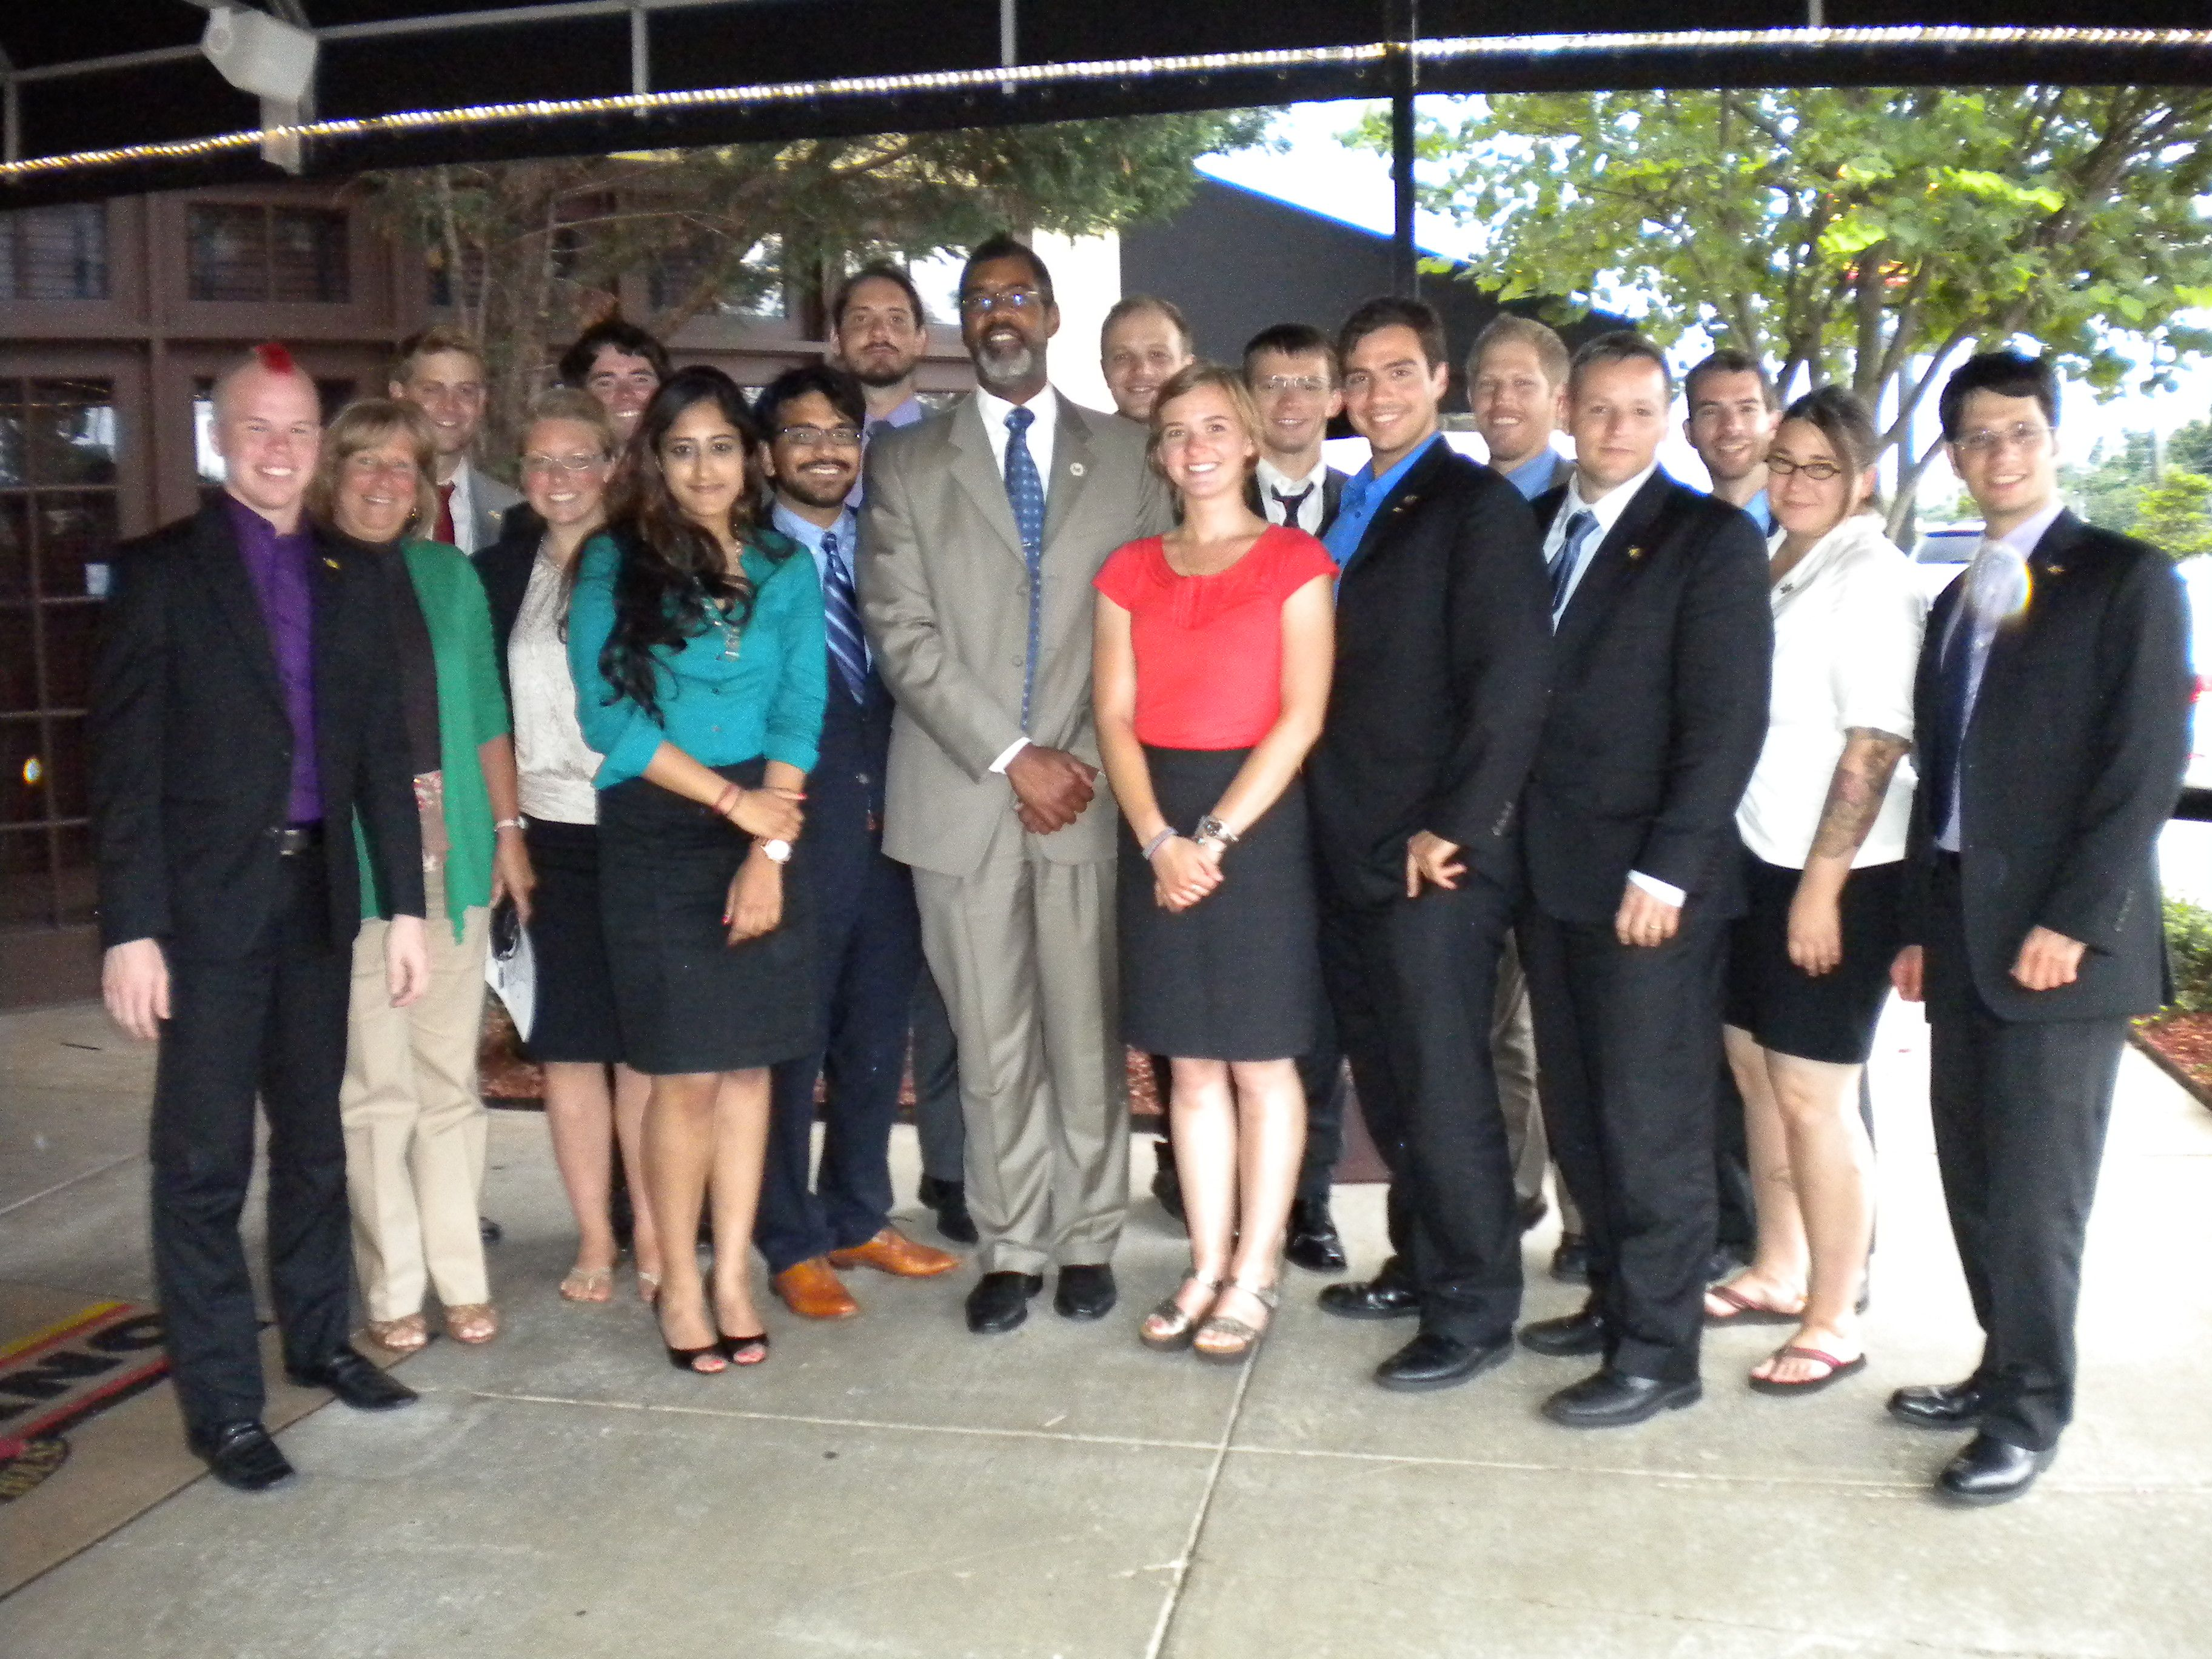
\includegraphics[scale=.4]{NESD_Mag.jpg} 
\end{figure}


\newpage
\section{Feedback for Next Year}

Most of the feedback from the delegates regarding the 2013 NESD was positive.  A
sampling of positive statements from the final Delegation meeting is included
here:

\begin{itemize}
\item The organization of this years Delegation received high praise
\item Preparation for key meetings, such as OMB, was much improved over the
  previous years Delegation
\item Delegates all thought that the meetings set up for the Delegation were
  outstanding and invaluable
\end{itemize}

Some ideas that were suggested for consideration are listed here:
\begin{itemize}
\item Delegates should be encouraged to contact their university Washington
  liaisons for advice and potential coordination with existing efforts.
\item Attempts should be made to set up meetings with Appropriations Committee
  staff.  Several delegates enthusiastically endorsed this idea.
\item An intro/preparatory meeting with a budget expert would be useful,
  especially for delegates not already familiar with the intricacies of the
  federal budget process.
\item An idea of having the Delegation extend from mid-week to mid-week rather
  than beginning on a weekend was raised.  This would allow for some of the
  preparatory meetings to occur before the statement-writing session.  Some
  delegates felt that information received at meetings could have been
  fruitfully incorporated into the statement-writing process.
\item For next years Delegation, formal thank you and follow-up letters could be
  sent to key people with whom the delegation meets.
\end{itemize}

Other suggestions focused on preparing future delegates, such as additions and
improvements to the Guidebook prepared this year.  The Guidebook was well
received, and the delegates found it useful.

All in all, the feedback from the delegates was that the 2013 Nuclear
Engineering Student Delegation was a success.  The delegates’ suggestions for
improvement focused on ways that next years delegation can be made even more
effective.  All delegates left the week with greatly increased understanding of
the importance of being involved in the legislative process, as well as renewed
passion for doing whatever they can to help support nuclear education programs.

\newpage
\section{Conclusion}

The 2013 Nuclear Engineering Student Delegation was very successful in educating
policymakers on the needs for supporting nuclear engineering education and the
members of the delegation on the political process. During the delegations time
in Washington, D.C., members were able to speak for nuclear science and
engineering students throughout the country and show their enthusiasm for
nuclear professions. This years delegation was fortunate to meet with some very
influential members and advocates of the nuclear community. The NESD was also
very successful on Capitol Hill as they were able to visit or meet with the
offices of numerous members of the House of Representatives and most sitting
members of the Senate during their time in Washington, D.C.

The primary goal of this year’s delegation was to express to policymakers the
need for the Integrated University Program (IUP) that provides fellowships and
scholarships through DOE/NE and NRC to nuclear science and engineering
students. Currently, the IUP has been funded under the House's Water \& Energy
Appropriations bill. It is still uncertain whether or not the senate will
include the IUP in their appropriations bill.p

All members of the 2013 NESD were very pleased with their experience in
Washington, D.C. Delegates who will be in school next year look forward to the
possibility of being part of the 2014 NESD, which will be chaired by Nicholas
Thompson (Rensselar Polytechnic Institute). Finally, the members of the
delegation would like to thank the Nuclear Energy Institute, American Nuclear
Society, and all of the universities of the delegates for their help and
support.

\end{document}
